% begin module limits-one-sided-ex6
\begin{frame}
\frametitle{One-sided Limits}
\begin{example}
\begin{columns}[c]
\column{.5\textwidth}
The Heaviside function $H$ is defined by
\[
H(x) = \left\{ \begin{array}{lr}
0 & \textrm{ if } x < 0\\
1 & \textrm{ if } x \geq 0
\end{array}\right. .
\]
\psset{xunit=1.1cm,yunit=1.1cm}
\begin{pspicture}(-2.5,-1.5)(2.5,1.5)
\psframe*[linecolor=white](-2.5, -1.5)(2.7, 1.7)
\psaxes[ticks=x, labels=none]{<->}(0,0)(-2.5,-1.5)(2.5,1.5)
\rput[b](0, 1.52){\tiny $y$}
\rput[l](2.52, 0){\tiny $x$}
\rput[r](-0.1,1){ $1$}
\psline[linecolor=red, linewidth=1pt](-2.5,0)(0,0)
\psline[linecolor=red, linewidth=1pt](0,1)(2.5,1)

\pscircle*[fillcolor=white, linecolor=red](0, 1){0.07}
\pscircle*[fillcolor=white, linecolor=red](0, 0){0.07}
\pscircle*[fillcolor=white, linecolor=white](0, 0){0.04}

\end{pspicture}
%\ 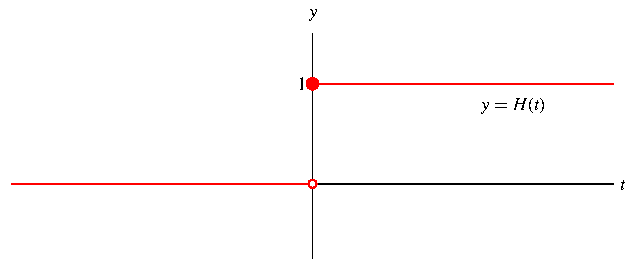
\includegraphics[height=2.5cm]{limits/pictures/02-02-ex6.pdf}%
\column{.5\textwidth}
\begin{itemize}
\item<2->  As $x$ approaches $0$ from the left, $H(x)$ approaches 0.
\item<3->  As $x$ approaches $0$ from the right, $H(x)$ approaches 1.
\item<4->  There is no single number that $H(x)$ approaches as $x$ approaches 0.
\item<5->  Therefore $\lim\limits_{x\rightarrow 0} H(x)$ doesn't exist.
\end{itemize}
\end{columns}
\end{example}
\end{frame}
% end module limits-one-sided-ex6
